\section{Análise de Resultados}
\label{sec:resultados}

Inicialmente, em nossas análises, via a pontuação normalizada de um conjunto de
aplicações, observamos que, de maneira geral, algumas aplicações tendem a
sofrer e a causar menos interferência do que outras aplicações. É o caso de
\textit{add\_double}, \textit{cachebench}, \textit{make} e \textit{povray}. Não
por acaso, são ferramentas que não possuem perfis de cargas de trabalho
voltados para operações de \textit{entrada/saída} ( \textit{add\_double} possui
perfil voltado para \textit{cpu}, \textit{make} e \textit{povray} possuem
perfil misto mas mais voltado para operações em \textit{cpu} do que de
\textit{entrada/saída} e \textit{cachebench} é mais voltado para operações no
sistema de memória). Assim, observamos também que essas aplicações, por
possuírem um perfil de carga de trabalho voltado mais para \textit{cpu} e
memória (no caso do \textit{cachebench}), praticamente não interferem em
aplicações que possuem um perfil voltado para \textit{operações de
entrada/saída} e nem mesmo sofrem interferência significativa desse tipo de
aplicações.

Por exemplo, observamos que a pontuação de \textit{povray} contra esse conjunto
de aplicações ficou próxima de 1 o que indica o grau de interferência bastante
insignificante, o mesmo ocorrendo com \textit{add\_double}. No caso do
\textit{cachebench}, mesmo tendo sido uma das ferramentas que menos sofreu
interferência, percebemos um grau de interferência mais elevado do que das
outras duas (\textit{povray} e \textit{add\_double}), isso se deve ao fato que
o sistema de memória acaba atuando principalmente em operações de
\textit{cache} tanto em aplicações com perfil voltado para \textit{cpu} quanto
em aplicações com perfil voltado para operações de \textit{entrada/saída}.

Para o restante das aplicações, observamos um grau de interferência maior e com
mais variações dependendo da aplicação que está sendo executada em
\textit{background}. Essas são típicas aplicações de \textit{entrada/saída},
com suas cargas de trabalho atuando em operações de escrita ou leitura em
disco. Por exemplo, observamos que o \textit{dd} e o \textit{cp} são as
aplicações que causam maior degradação no desempenho das aplicações voltadas
para \textit{entrada/saída}. Dessa forma, em uma das combinações realizadas,
executando \textit{Bzip2} contra \textit{dd}, a pontuação ficou abaixo de 0.4,
evidenciando um elevado grau de degradação.

Dada a variação de interferência de desempenho entre essas aplicações,
destacamos que a pontuação alcançada de \textit{gzip} e \textit{bzip2} contra
\textit{grep} indica um grau de degradação de desempenho pequeno ou
praticamente nulo. Em contrapartida, a pontuação alcançada por \textit{cp},
\textit{cat} e \textit{dd} contra \textit{grep} mostra uma degradação do
desempenho maior se comparada com \textit{gzip} e \textit{bzip2} contra
\textit{grep}. Em suma, isso indica que mesmo dentre as aplicações típicas de
\textit{entrada/saída} pode haver um padrão de interferência dado o seu tipo de
execução (escrita ou leitura). 

Posteriormente, aplicamos os mecanismos de predição baseados nos dados
coletados via as métricas de desempenho em nível de sistema e da pontuação
normalizada das aplicações. Com isso, esperamos predizer a pontuação
normalizada de uma aplicação a partir dos valores alcançados nas métricas de
desempenho a nível de sistema. 

\begin{figure}[!htb]
\centering
\includegraphics [keepaspectratio=true,scale=0.5]{graficos/mean_predict.eps}
\caption{Comparativo entre a pontuação normalizada real e a pontuação predita utilizando média ponderada com o aúxilio da análise por componente principal.}
\label{mean_predict}
\end{figure}   

A Figura \ref{mean_predict} apresenta um comparativo dos resultados alcançados
utilizando a média ponderada com os valores reais da pontuação normalizada.
Observa-se que no geral de fato o modelo é capaz de predizer com certa
precisão. Observa-se, por exemplo, Bzip2 @ Bzip2 e Crypt @ Cat que os erros de
predição obtidos foram 0,68\% e 0,13\% respectivamente. Entretanto, há alguns
casos que há uma discrepância relevante como por exemplo Crypt @ Grep ao qual o
erro de predição foi de 41,5\%.
   

\begin{figure}[!htb]
\centering
\includegraphics [keepaspectratio=true,scale=0.5]{graficos/linear.eps}
\caption{Comparativo entre a pontuação normalizada real e a pontuação predita utilizando regressão linear.}
\label{linear_predict}
\end{figure}   

A Figura \ref{linear_predict} apresenta os resultados da predição utilizando
regressão linear. Nota-se que em muitos casos os valores preditos pela
regressão linear possuem uma diferença maior para os valores reais do que na
predição feita por média ponderada. Assim, enquanto que Gzip @ Cat e bzip2 @ cp
obteve uma taxa de erro de 7,92\% e 1 ,65\% respectivamente na predição
utilizando média ponderada, na análise de regressão linear esse valores foram
de 53,6\% e 31,4\%. Mas ainda assim, para alguns casos, o modelo de regressão
linear conseguiu prever com uma taxa de erro mais baixa como por exemplo em dd
@ gzip e crypt @ cat, em que as taxas de erros da predição foram de 1,25\% e
5,67\% respectivamente.

Nos resultados apresentados na Figura \ref{poli_predict} percebe-se que dentre
os três modelos, a regressão polinomial é a que obtém valores de predição com
menores taxas de erro. Assim, enquanto que Crypt @ Grep obteve uma taxa de erro
de 41,5\% utilizando a média ponderada como modelo de predição, na análise de
regressão polinomial essa taxa de erro foi de 3,92\%. Dentre os resultados
apresentados na Figura \ref{poli_predict}, Cat @ dd foi o que obteve maior taxa
de erro, 19,5\%. 

\begin{figure}[!htb]
\centering
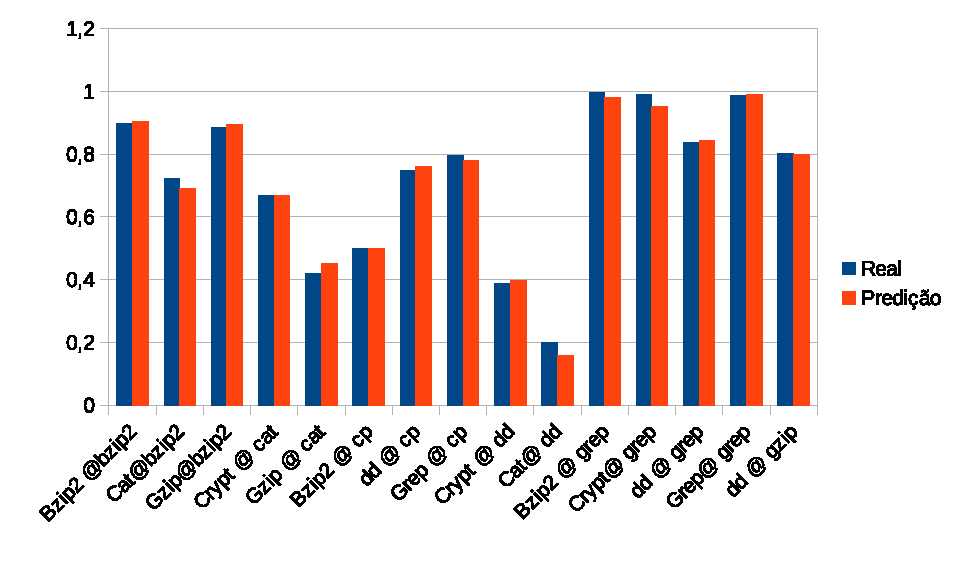
\includegraphics [keepaspectratio=true,scale=0.5]{graficos/poli.eps}
\caption{Comparativo entre a pontuação normalizada real e a pontuação predita utilizando regressão polinomial.}
\label{poli_predict}
\end{figure}  

A partir disso, a fim de verificar a qualidade dos modelos de regressão
aplicados, foi calculado o coeficiente de determinação R\textsuperscript{2}
tanto para a regressão linear quanto para a regressão polinomal. Dessa forma, a
regressão linear apresentou um coeficiente de determinação de 80,3\% enquanto
que a regressão polinomial atingiu um índice de 96,6\%, demonstrando que assim
como havia sido observado nos gráficos de predição, que a regressão polinomial
é o modelo mais adequado para a predição de desempenho dos dados se comparada
com a regressão linear.   

Como comparativo para os três modelos de predição foram calculados a média,
mediana e o maior erro de predição para todos os modelos. As Figuras
\ref{mean_error}, \ref{linear_error} e \ref{polinomial_error} apresenta esses
resultados.

\begin{figure}[!htb]
\centering
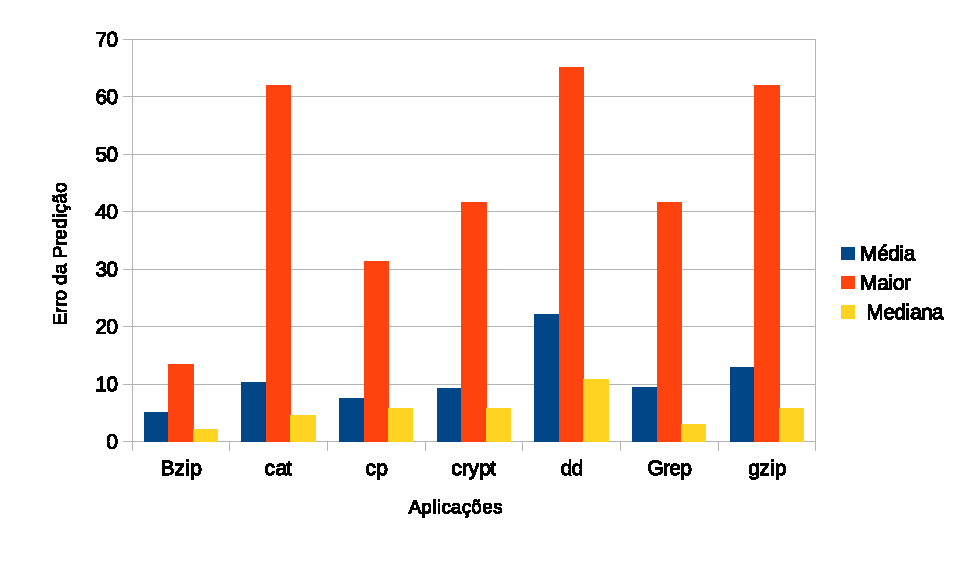
\includegraphics [keepaspectratio=true,scale=0.5]{graficos/mean_error.eps}
\caption{Média, mediana e erro máximo da predição de desempenho com o método da média ponderada}
\label{mean_error}
\end{figure}  

\begin{figure}[!htb]
\centering
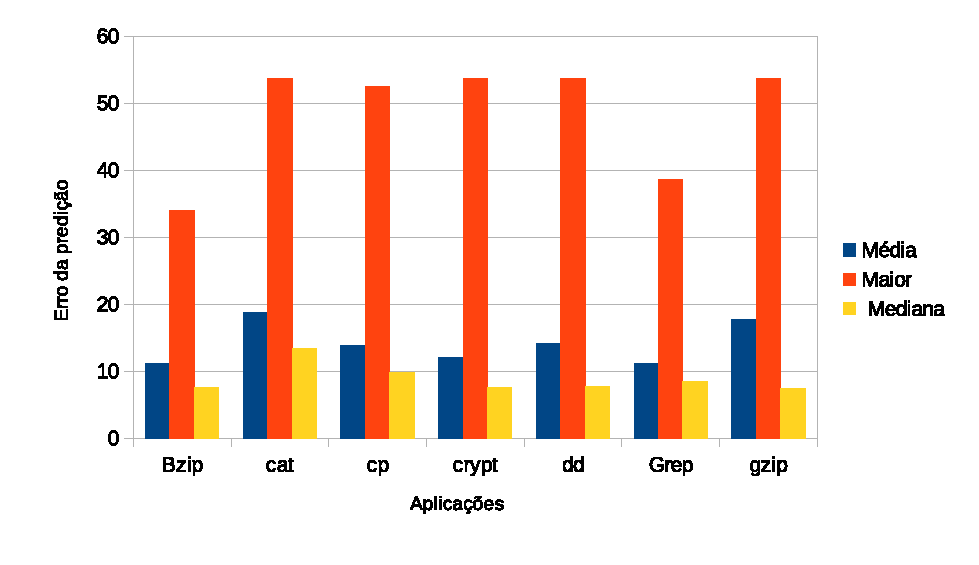
\includegraphics[width=.5\textwidth]{graficos/linear_error.eps}
\caption{Média, mediana e erro máximo da predição de desempenho com regressão linear}
\label{linear_error}
\end{figure}  

\begin{figure}[!htb]
\centering
\includegraphics[width=.5\textwidth]{graficos/polinomial_error.eps}
\caption{Média, mediana e erro máximo da predição de desempenho com regressão polinomial}
\label{polinomial_error}
\end{figure}  


Assim como no trabalho de Koh \cite{koh2007}, comparada à média ponderada, a
regressão linear apresenta resultados inferiores relacionados a predição, com a
média de erros para todos os dados de 13,5\% e mediana de 8,8\%. Isso pode
estar relacionado ao fato da correlação entre as métricas de desempenho em
nível de sistema e a pontuação normalizada de uma aplicação não ser linear
\cite{koh2007}. Dessa forma, a regressão polinomial foi aplicada neste
trabalho. Além dos dados apresentados na Figura \ref{poli_predict} e no cálculo
do coeficiente de determinação R \textsuperscript{2}, os valores da média,
mediana e erro máximo apresentados na Figura \ref{polinomial_error} demonstram
que a regressão polinomial obtém resultados melhores para predição se comparada
com os modelos anteriores. Assim, de maneira geral, a média de erro para todos
os resultados alcançou um valor de 5\% e de mediana 2,7\%.

